\documentclass[10pt]{article}

\usepackage[T1]{fontenc}
\usepackage{geometry}
\usepackage{amsmath, amssymb, amsthm}
\usepackage{listings}
\usepackage{graphicx}
\usepackage{float}
\usepackage{bm}
\usepackage{hyperref}

\geometry{a4paper, margin=1in}

\renewcommand{\labelenumi}{(\alph{enumi})}
\renewcommand{\vec}{\bm}

\renewcommand{\C}{\mathbb{C}}
\newcommand{\R}{\mathbb{R}}
\newcommand{\Q}{\mathbb{Q}}
\newcommand{\Z}{\mathbb{Z}}
\newcommand{\N}{\mathbb{N}}

\setlength{\parindent}{0em}

\title{Assignment II}
\author{Satvik Saha}
\date{}

\begin{document}
    \noindent\textbf{IISER Kolkata} \hfill \textbf{Assignment II}
    \vspace{3pt}
    \hrule
    \vspace{3pt}
    \begin{center}
    \LARGE{\textbf{MA4106: Statistics II}}
    \end{center}
    \vspace{3pt}
    \hrule
    \vspace{3pt}
    Satvik Saha, \texttt{19MS154} \hfill \today
    \vspace{20pt}

    \setlength{\parskip}{1em}



    \section{Model selection}

    We return to the Boston Housing dataset, and examine the variation of
    \texttt{LOGMEDV} (the logarithm of the median value of homes in \$1000's) with 13
    related variables. If we are willing to perform linear regression using only a
    subset of our independent variables, there are $2^{13} = 8192$ models to
    consider and compare. Here, we use the Akaike Information Criterion (AIC) to
    compare two models, calculated as \[
        \text{AIC} = n\log\left(\frac{\text{RSS}}{n}\right) + 2K,
    \] where the given model has $K$ parameters, fitted on a dataset of size $n$, and
    gives a residual sum of squares error RSS. Better models have lower AIC.

    \textit{Remark: In this particular case, our dataset is fairly small, allowing us
    to brute force all $8192$ models relatively quickly. A summary of the best 5
    models (by AIC) is given below. Here, $\Delta\text{AIC}$ denotes the difference
    between the AIC and the smallest AIC in the list. Note that the model with all 13
    parameters ranks fifth.}

    \begin{table}[H]
        \centering
        \caption{Best models (brute force)}
        \vspace{0.8em}
        \label{tab:models_all}
        \begin{tabular}{|c|c|c|c|l|} \hline
            $K$ & $R^2$ & $R^2_{adj}$ & $\Delta$AIC & Features \\\hline
            11& 0.7891& 0.7844& 0.0000& \footnotesize\texttt{CRIM}, \texttt{ZN}, \texttt{CHAS}, \texttt{NOX}, \texttt{RM}, \texttt{DIS}, \texttt{RAD}, \texttt{TAX}, \texttt{PTRATIO}, \texttt{B}, \texttt{LSTAT} \\
            12& 0.7896& 0.7845& 0.9676& \footnotesize\texttt{CRIM}, \texttt{ZN}, \texttt{INDUS}, \texttt{CHAS}, \texttt{NOX}, \texttt{RM}, \texttt{DIS}, \texttt{RAD}, \texttt{TAX}, \texttt{PTRATIO}, \texttt{B}, \texttt{LSTAT} \\
            12& 0.7892& 0.7841& 1.8363& \footnotesize\texttt{CRIM}, \texttt{ZN}, \texttt{CHAS}, \texttt{NOX}, \texttt{RM}, \texttt{AGE}, \texttt{DIS}, \texttt{RAD}, \texttt{TAX}, \texttt{PTRATIO}, \texttt{B}, \texttt{LSTAT} \\
            10& 0.7874& 0.7831& 2.1086& \footnotesize\texttt{CRIM}, \texttt{CHAS}, \texttt{NOX}, \texttt{RM}, \texttt{DIS}, \texttt{RAD}, \texttt{TAX}, \texttt{PTRATIO}, \texttt{B}, \texttt{LSTAT} \\
            13& 0.7896& 0.7841& 2.8044& \footnotesize\texttt{CRIM}, \texttt{ZN}, \texttt{INDUS}, \texttt{CHAS}, \texttt{NOX}, \texttt{RM}, \texttt{AGE}, \texttt{DIS}, \texttt{RAD}, \texttt{TAX}, \texttt{PTRATIO}, \texttt{B}, \texttt{LSTAT} \\\hline
        \end{tabular}
    \end{table}

    We can also adopt the following stepwise procedures.

    \begin{enumerate}
        \item \textbf{Forward selection:} Start with a model without any independent
        variables, and create $K$ models each with a single parameter $\beta_i$. For
        each, test the hypothesis $\beta_i \neq 0$ against the null hypothesis
        $\beta_i = 0$ using an $F$-test, and choose the model with the best (highest)
        $F$-score (indicating that the corresponding $\beta_i$ is significant).
        Repeat the above, adding parameters one by one until the $F$-scores are not
        significantly high, i.e.\ all $F$-scores are below some threshold $F_{in}$.

        \item \textbf{Backward elimination:} Start with a model with all $K$
        independent variables, and create $K$ models each removing a single parameter
        $\beta_i$. For each, test the hypothesis $\beta_i \neq 0$ against the null
        hypothesis $\beta_i = 0$ using an $F$-test, and choose the model with the
        worst (lowest) $F$-score (indicating that the corresponding $\beta_i$ is not
        significant).  Repeat the above, removing parameters one by one until the
        $F$-scores become significantly high, i.e.\ all $F$-scores are above some
        threshold $F_{out}$.

        \item \textbf{Forward-backward}: Start with an empty model, then perform
        alternating forward selection and backward elimination steps, adding and
        removing variables based on thresholds $F_{in}$ and $F_{out}$
    \end{enumerate}

    Below are the results of these three selection procedures, using thresholds
    $F_{out} = 1.0, F_{in} = 2.0$.

    \begin{table}[H]
        \centering
        \caption{Best models (stepwise selection)}
        \vspace{0.8em}
        \label{tab:models_all}
        \begin{tabular}{|l|c|c|c|l|} \hline
            Procedure & $K$ & $R^2_{adj}$ & $\Delta$AIC & Features \\\hline
            Forward          &  11& 0.7844& 0.0000  &\footnotesize\texttt{LSTAT}, \texttt{PTRATIO}, \texttt{CRIM}, \texttt{RM}, \texttt{DIS}, \texttt{NOX}, \texttt{B}, \texttt{RAD}, \texttt{TAX}, \texttt{CHAS}, \texttt{ZN} \\
            Forward-Backward &  11& 0.7844& 0.0000  &\footnotesize\texttt{LSTAT}, \texttt{PTRATIO}, \texttt{CRIM}, \texttt{RM}, \texttt{DIS}, \texttt{NOX}, \texttt{B}, \texttt{RAD}, \texttt{TAX}, \texttt{CHAS}, \texttt{ZN} \\
            Backward         &  12& 0.7845& 0.9676  &\footnotesize\texttt{DIS}, \texttt{PTRATIO}, \texttt{CRIM}, \texttt{CHAS}, \texttt{RAD}, \texttt{B}, \texttt{TAX}, \texttt{RM}, \texttt{LSTAT}, \texttt{ZN}, \texttt{INDUS}, \texttt{NOX} \\
            OLS              &  13& 0.7841& 2.8044  &\footnotesize\texttt{CRIM}, \texttt{ZN}, \texttt{INDUS}, \texttt{CHAS}, \texttt{NOX}, \texttt{RM}, \texttt{AGE}, \texttt{DIS}, \texttt{RAD}, \texttt{TAX}, \texttt{PTRATIO}, \texttt{B}, \texttt{LSTAT} \\\hline
        \end{tabular}
    \end{table}

    We see that both the forward and the forward-backward procedures select the
    `best' model with 11 variables. Note that the features for these two rows in the
    table are presented in order of addition. The backward elimination procedure
    produces the next best model with 12 variables; the variable \texttt{INDUS} is
    not eliminated. \emph{This model has a slightly better $R^2_{adj}$ than the
    remaining ones.}

    Here is the output for the backward elimination process. Each line represents a
    model with the indicated variable removed. Here, \texttt{D\_AIC} represents the
    difference between the AIC of the new model with the existing model; a negative
    value indicates an improvement.

    \lstset{basicstyle=\ttfamily\footnotesize,breaklines=true}
    \begin{lstlisting}
    Backward Elimination
    Current model uses features ['CRIM', 'ZN', 'INDUS', 'CHAS', 'NOX', 'RM', 'AGE', 'DIS', 'RAD', 'TAX', 'PTRATIO', 'B', 'LSTAT']
    -AGE        => F =   0.1587, p = 0.6906, adjR2 =   0.7845, D_AIC =  -1.8369
    -INDUS      => F =   1.0043, p = 0.3168, adjR2 =   0.7841, D_AIC =  -0.9681
    -ZN         => F =   4.5533, p = 0.0333, adjR2 =   0.7825, D_AIC =   2.6613
    -CHAS       => F =   8.5584, p = 0.0036, adjR2 =   0.7808, D_AIC =   6.7263
    -B          => F =  14.7979, p = 0.0001, adjR2 =   0.7780, D_AIC =  12.9946
    -TAX        => F =  17.2838, p = 0.0000, adjR2 =   0.7770, D_AIC =  15.4705
    -NOX        => F =  25.9206, p = 0.0000, adjR2 =   0.7732, D_AIC =  23.9797
    -RAD        => F =  28.8640, p = 0.0000, adjR2 =   0.7719, D_AIC =  26.8471
    -RM         => F =  29.4849, p = 0.0000, adjR2 =   0.7716, D_AIC =  27.4500
    -DIS        => F =  37.8059, p = 0.0000, adjR2 =   0.7680, D_AIC =  35.4602
    -PTRATIO    => F =  53.4154, p = 0.0000, adjR2 =   0.7611, D_AIC =  50.1529
    -CRIM       => F =  60.9695, p = 0.0000, adjR2 =   0.7578, D_AIC =  57.1130
    -LSTAT      => F = 204.5929, p = 0.0000, adjR2 =   0.6949, D_AIC = 173.9476
    Removed AGE       

    Current model uses features ['CRIM', 'ZN', 'INDUS', 'CHAS', 'NOX', 'RM', 'DIS', 'RAD', 'TAX', 'PTRATIO', 'B', 'LSTAT']
    -INDUS      => F =   1.0069, p = 0.3161, adjR2 =   0.7844, D_AIC =  -0.9676
    -ZN         => F =   4.4223, p = 0.0360, adjR2 =   0.7830, D_AIC =   2.5187
    -CHAS       => F =   8.7145, p = 0.0033, adjR2 =   0.7811, D_AIC =   6.8661
    -B          => F =  15.0808, p = 0.0001, adjR2 =   0.7783, D_AIC =  13.2464
    -TAX        => F =  17.2296, p = 0.0000, adjR2 =   0.7774, D_AIC =  15.3819
    -NOX        => F =  26.7816, p = 0.0000, adjR2 =   0.7732, D_AIC =  24.7672
    -RAD        => F =  28.7545, p = 0.0000, adjR2 =   0.7723, D_AIC =  26.6841
    -RM         => F =  31.7976, p = 0.0000, adjR2 =   0.7710, D_AIC =  29.6267
    -DIS        => F =  42.9588, p = 0.0000, adjR2 =   0.7661, D_AIC =  40.2753
    -PTRATIO    => F =  53.3780, p = 0.0000, adjR2 =   0.7616, D_AIC =  50.0178
    -CRIM       => F =  61.0536, p = 0.0000, adjR2 =   0.7582, D_AIC =  57.0767
    -LSTAT      => F = 227.5439, p = 0.0000, adjR2 =   0.6856, D_AIC = 190.0256

    Final model uses 12 features ['ZN', 'INDUS', 'NOX', 'DIS', 'PTRATIO', 'CHAS', 'RM', 'TAX', 'B', 'LSTAT', 'CRIM', 'RAD']
    \end{lstlisting}

    We see that in the final pass, the $F$-score for the model without \texttt{INDUS}
    remains above the threshold $F_{out}$, even though the corresponding $p$-value is
    fairly high. Indeed, when using $p$-values to test hypotheses instead of the
    static $F$-score thresholds (note that the degrees of freedom change on each
    pass), all three methods produce the same 11 variable model (with a level of
    significance $0.05$). With this, there seems to be no significant difference
    between the three procedures, apart from the number of iterations taken to reach
    the final model. The backward elimination model finishes much faster than the
    rest here, since the majority of variables here are significant; this may not
    always be the case if the available variables are not as suitable.

    The code used to generate these models, as well as the output (using $p$-values,
    level of significance $\alpha = 0.05$) has been attached.

    \textit{From the procedure outputs, we see that all algorithms seem to follow the
    `path of least AIC', i.e.\ among the available new models, the one with the
    greatest AIC drop is chosen. The procedure terminates when none of the new models
    offer an improvement via a drop in AIC.}


    \begin{table}[H]
        \centering
        \caption{Parameter estimates using the models from Table 2.}
        \vspace{0.8em}
        \label{tab:models_parameters}
        \begin{tabular}{|r|r|r|r|} \hline
                 Parameter &  $k = 11$ &  $k = 12$ &  $k = 13$ \\\hline
                 $\beta_0$ &    4.0837 &    4.0952 &    4.1020 \\
             \texttt{CRIM} &   -0.0103 &   -0.0103 &   -0.0103 \\
               \texttt{ZN} &    0.0011 &    0.0011 &    0.0012 \\
            \texttt{INDUS} &       --- &    0.0025 &    0.0025 \\
             \texttt{CHAS} &    0.1051 &    0.1016 &    0.1009 \\
              \texttt{NOX} &   -0.7217 &   -0.7623 &   -0.7784 \\
               \texttt{RM} &    0.0907 &    0.0922 &    0.0908 \\
              \texttt{AGE} &       --- &       --- &    0.0002 \\
              \texttt{DIS} &   -0.0517 &   -0.0500 &   -0.0491 \\
              \texttt{RAD} &    0.0134 &    0.0142 &    0.0143 \\
              \texttt{TAX} &   -0.0006 &   -0.0006 &   -0.0006 \\
          \texttt{PTRATIO} &   -0.0374 &   -0.0381 &   -0.0383 \\
                \texttt{B} &    0.0004 &    0.0004 &    0.0004 \\
            \texttt{LSTAT} &   -0.0286 &   -0.0288 &   -0.0290 \\\hline
        \end{tabular}
    \end{table}




    \section{Bootstrap methods}

    Given a table of $n = 15$ schools, each with an \texttt{LSAT} and a \texttt{GPA}
    score, we can calculate the correlation between these two columns as $\rho =
    0.748$. To estimate the standard error, we use the bootstrap procedure of drawing
    $B$ random samples with replacement, each consisting of $15$ rows from the data
    table. We calculate the correlation $\rho_i$ between the \texttt{LSAT} and
    \texttt{GPA} for each sample $1 \leq i \leq B$, and thus obtain a bootstrap
    distribution $\hat{f}_B$ for the correlation. Using this, we calculate an
    estimate of the standard error \[
        [\hat{\text{se}}_B(\rho)]^2 =
        \frac{1}{B - 1} \sum_{i = 1}^B (\rho_i - \bar{\rho})^2.
    \] The probability that $\rho > 0.5$ can be estimated from this distribution
    as \[
        \frac{1}{B}\sum_{i = 1}^B I_{(0.5, 1]}(\rho_i),
    \] i.e.\ the proportion of bootstrap estimates $\rho_i$ that are above $0.5$.

    We perform these calculations for $25 \leq B \leq 3000$ (reusing samples from the
    previous $B$) and obtain the following variation of the estimate of
    $\text{se}_B(\rho)$.


    \begin{figure}[H]
    \begin{center}
        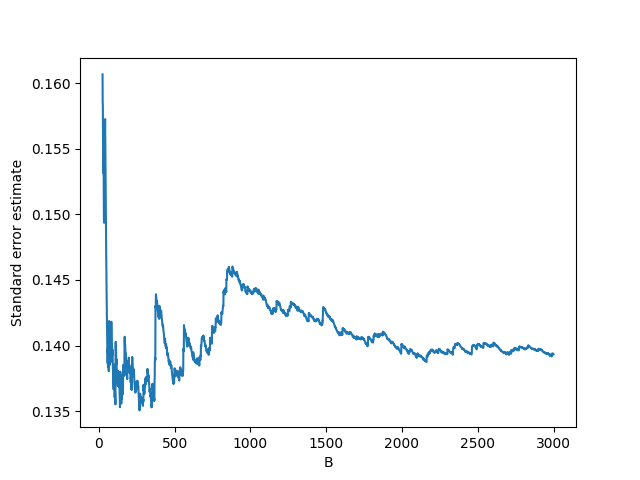
\includegraphics[width=0.8\textwidth]{bootstrap/errors.png}
    \end{center}
    \caption{Variation of $\hat{\text{se}}_{B}(\rho)$ with $B$}
    \label{fig:bootstrap_error}
    \end{figure}

    The final estimate of the standard error is $0.139$ ($B = 3000$).

    \begin{figure}[H]
    \begin{center}
        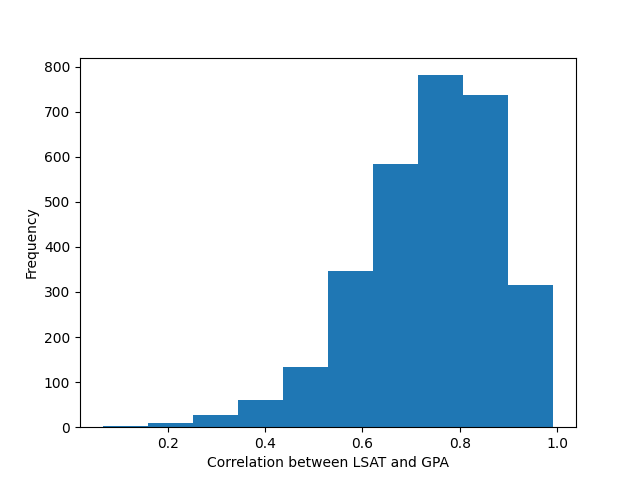
\includegraphics[width=0.8\textwidth]{bootstrap/correlations.png}
    \end{center}
    \caption{Histogram of the 3000 bootstrap estimates $\rho_i$.}
    \label{fig:bootstrap_error}
    \end{figure}

    The estimate of $P(\rho > 0.5)$ is $0.942$.


\end{document}
